\section{1174006 - Kadek Diva Krishna Murti}

\subsection{Teori}
\begin{enumerate}
	\item Jelaskan kenapa file suara harus di lakukan MFCC. dilengkapi dengan ilustrasi atau gambar.
	\hfill\break
	Mel Frequency Cepstral Coefficient (MFCC) untuk ekstraksi ciri yang akan mengubah deretan nilai amplitudo menjadi frame-frame yang kemudian akan diolah menggunakan mel-filterbank yang mengadaptasi cara kerja pendengaran manusia sehingga terbentuklah nilai-nilai koefisien yang menjadi fitur ciri sehingga dapat membedakan suara satu dengan suara lainnya.
	\hfill\break
	\begin{figure}[H]
		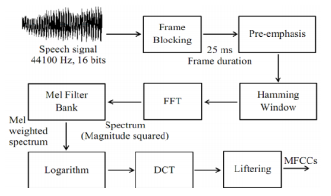
\includegraphics[width=8cm]{figures/1174006/chapter6/teori/mfcc.png}
		\centering
	\end{figure}
	\item Jelaskan konsep dasar neural network.dilengkapi dengan ilustrasi atau gambar.
	\hfill\break
	\begin{itemize}
		\item Sejumlah sinyal masukan (x) dikalikan dengan masing-masing weight (W) 
		\item Kemudian dilakukan penjumlahan dari seluruh hasil perkalian tersebut dan keluaran yang dihasilkan diteruskan ke fungsi activation untuk mendapatkan tingkatan derajat sinyal keluarannya (F(x.W))
		\item Walaupun masih jauh dari sempurna, namun kinerja dari tiruan neuron ini identik dengan kinerja dari sel otak.
	\end{itemize}
	\hfill\break
	\begin{figure}[H]
		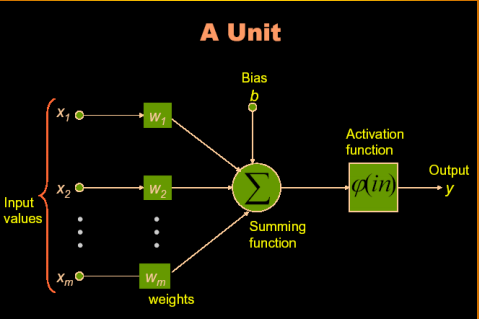
\includegraphics[width=8cm]{figures/1174006/chapter6/teori/neuron.png}
		\centering
	\end{figure}
	\item Jelaskan konsep pembobotan dalam neural network. dilengkapi dengan ilustrasi atau gambar.
	\hfill\break
	Weight digunakan untuk menghubungkan setiap neuron dalam satu lapisan ke setiap neuron di lapisan berikutnya. Weight menentukan kekuatan koneksi antara neuron. Weights sangat krusial bagi neuron, karena ini merupakan bagian agar neuron bisa belajar. Nilai w (simbol untuk weights) bisa sama dan bisa juga tidak untuk setiap input yang diterima dari neuron. Semakin besar nilai w sebuah input, maka sinyal yang berasal dari input tertentu memiliki prioritas yang semakin besar untuk bisa berkontribusi kepada neuron di depannya. Selain itu, nilai w juga menentukan apakah sinyal dari input tertentu bisa melewati neuron di depannya atau tidak.
	\item Jelaskan konsep fungsi aktifasi dalam neural network.  dilengkapi dengan ilustrasi atau gambar.
	\hfill\break
	Fungsi activation adalah untuk memutuskan apakah neuron harus diaktifkan atau tidak dengan menghitung jumlah weight dan selanjutnya menambahkan bias. Tujuan dari fungsi aktivasi adalah untuk memperkenalkan non-linearitas ke dalam output neuron. Contoh jaringan saraf memiliki neuron yang bekerja dalam korespondensi weight, bias dan fungsi aktivasi masing-masing. Dalam jaringan saraf, kita akan memperbarui bobot dan bias neuron berdasarkan kesalahan pada output. Proses ini dikenal sebagai back-propagation. Fungsi aktivasi memungkinkan back-propagation karena gradien diberikan bersama dengan kesalahan untuk memperbarui bobot dan bias.
	\item Jelaskan cara membaca hasil plot dari MFCC, dilengkapi dengan ilustrasi atau gambar.
	\hfill\break
	\begin{figure}[H]
		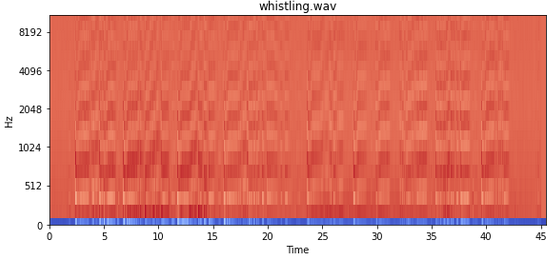
\includegraphics[width=8cm]{figures/1174006/chapter6/praktek/1-2.png}
		\centering
	\end{figure}
	Sumbu y untuk tinggi rendah frekuensi dan sumbu x untuk lama waktu audionya. Semakin gelap warnanya, atau semakin dekat ke merah, semakin banyak daya dalam rentang frekuensi pada waktu itu.
	\item Jelaskan apa itu one-hot encoding, dilengkapi dengan  ilustrasi kode dan atau gambar.
	\hfill\break
	one-hot encoding merupakan proses untuk mengkoversi variable categorical menjadi bentuk yang dapat diterapkan untuk ML. Contoh motor = 0, mobil = 1, dan seterusnya.
	\item Jelaskan apa fungsi dari np.unique dan to\_categorical dalam kode program, dilengkapi dengan ilustrasi atau gambar.
	\hfill\break
	Fungsi np.unique adalah untuk mengembalikan array elemen unik dari inputan array. Contoh sebuah array [5, 2, 6, 2, 7, 5, 6, 8, 2, 9] diterapkan fungsi np.unique hasilnya menjadi [2, 5, 6, 7, 8, 9].
	Fungsi to\_categorical adalah untuk mengubah nama class menjadi beberapa genre atau mengkategorikan class sesuai jenisnya. Contoh 0 = motor, 1 = mobil, dan seterusnya.
	\item Jelaskan apa fungsi dari Sequential dalam kode program,dilengkapi dengan ilustrasi atau gambar.
	\hfill\break
	Fungsi dari Sequential adalah untuk memodelkan atau membuat prediksi jenis data yang sequential atau berurutan, seperti audio, teks, dan lain-lain. Contoh program untuk mengambil sepotong teks dalam bahasa Indonesia dan menerjemahkannya ke bahasa Inggris.
\end{enumerate}

\subsection{Praktek}
\begin{enumerate}
	\item Jelaskan isi dari data GTZAN Genre Collection dan data dari freesound. Buat kode program untuk meload data tersebut untuk digunakan pada MFCC. Jelaskan arti dari setiap baris kode yang dibuat(harus beda dengan teman sekelas).
	\hfill\break
	Data GTZAN Genre Collection berisikan 1000 lagu dari 10 genre berbeda. Di tiap genrenya masing-masing terdapat 100 lagu yang kurang lebih durasinya 30 detik.\\
	Data dari freesound ada dua, yaitu Kick Loop 5 dan Whistling. Kick Loop 5 merupakan lagu dengan beat bass rendah sedangkan Whistling merupakan lagu yang bernada tinggi.\\
	Kode program untuk meload data tersebut untuk digunakan pada MFCC.
	\lstinputlisting[firstline=2, lastline=10]{src/1174006/chapter6/praktek/1.py}
	Import library librosa untu mengekstrak fitur dari lagu, import library glob untuk me-list file lagu ke berbagai direktori genre, import library numpy untuk melakukan operasi numerical, import library matplotlib untuk menggambar grafik MFCC, import model sequential dari library keras, import layer dense dari library keras yang memiliki banyak neuron di dalamnya, import layer activation dari library keras untuk menggunakan activation function di tiap layer neuron, dan import to\_categorical dari library keras untuk mengubah nama class menjadi beberapa genre.
	\lstinputlisting[firstline=12, lastline=21]{src/1174006/chapter6/praktek/1.py}
	Membuat fungsi untuk menampilkan nilai dari MFCC dari tiap lagu. Pertama load lagunya, lalu ekstrak lagunya dengan fungsi mfcc dan tampung nilainya. Kemudian tampilkan spectogramnya dengan fungsi specshow.
	\lstinputlisting[firstline=23, lastline=23]{src/1174006/chapter6/praktek/1.py}
	Ini spectogram dari Kick Loop 5 yang menampilkan frekuensi rendah.
	\hfill\break
	\begin{figure}[H]
		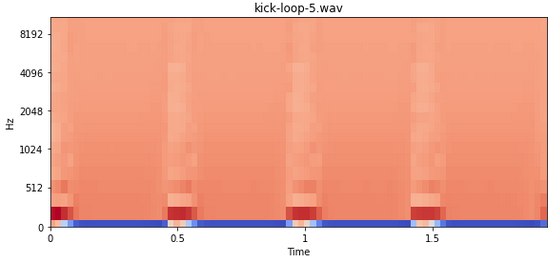
\includegraphics[width=8cm]{figures/1174006/chapter6/praktek/1-1.png}
		\centering
	\end{figure}
	\lstinputlisting[firstline=25, lastline=25]{src/1174006/chapter6/praktek/1.py}
	Ini spectogram dari Whistling yang menampilkan frekuensi tinggi.
	\hfill\break
	\begin{figure}[H]
		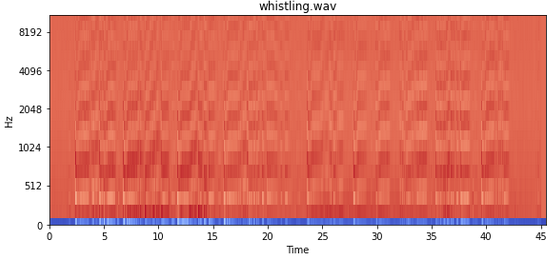
\includegraphics[width=8cm]{figures/1174006/chapter6/praktek/1-2.png}
		\centering
	\end{figure}
	\lstinputlisting[firstline=27, lastline=27]{src/1174006/chapter6/praktek/1.py}
	Ini spectogram dari lagu genre disco.
	\hfill\break
	\begin{figure}[H]
		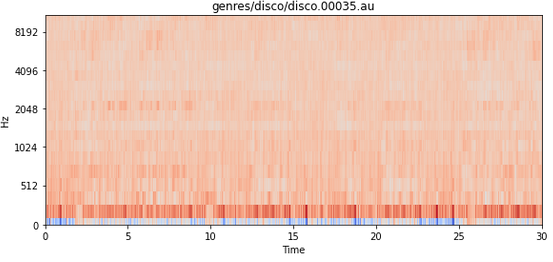
\includegraphics[width=8cm]{figures/1174006/chapter6/praktek/1-3.png}
		\centering
	\end{figure}
	\lstinputlisting[firstline=29, lastline=29]{src/1174006/chapter6/praktek/1.py}
	Ini spectogram dari lagu genre classical.
	\hfill\break
	\begin{figure}[H]
		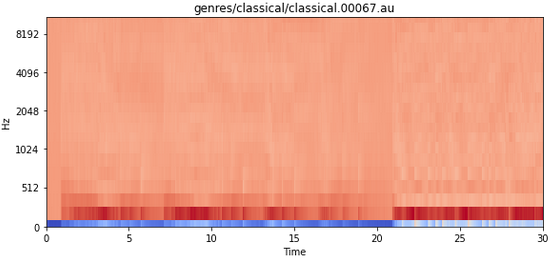
\includegraphics[width=8cm]{figures/1174006/chapter6/praktek/1-4.png}
		\centering
	\end{figure}
	\item Jelaskan perbaris kode program dengan kata-kata dan dilengkapi ilustrasi gambar fungsi dari display\_mfcc()
	\hfill\break
	Kode fungsi display\_mfcc()
	\lstinputlisting[firstline=2, lastline=11]{src/1174006/chapter6/praktek/2.py}
	\begin{itemize}
		\item Disini nama fungsinya display\_mfcc() dengan parameter song untuk lagu yang nantinya diproses.
		\item Panggil fungsi load() untuk meload lagunya kemudian ditampung nilainya.
		\item Panggil fungsi mfcc() untuk mengekstrak fitur dari lagunya kemudian ditampung nilainya.
		\item Panggil fungsi figure() untuk membuat grafiknya.
		\item Panggil fungsi specshow() untuk membuat spectogramnya
		\item Panggil fungsi colorbar() untuk memberi warna pada grafiknya.
		\item Panggil fungsi title() untuk memberi judul pada grafiknya.
		\item Panggil fungsi tight\_layout() untuk menyesuaikan grafiknya sesuai layout.
		\item Panggil fungsi show() untuk menampilkan grafiknya.
	\end{itemize}
	Jika kita memanggil fungsi display\_mfcc() nantinya akan seperti ini.
	\hfill\break
	\begin{figure}[H]
		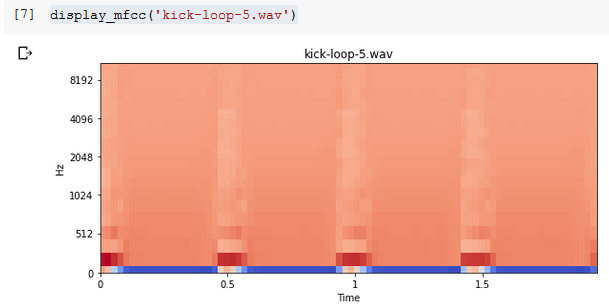
\includegraphics[width=8cm]{figures/1174006/chapter6/praktek/2-1.png}
		\centering
	\end{figure}
	\item Jelaskan perbaris kode program dengan kata-kata dan dilengkapi ilustrasi gambar fungsi dari extract\_features\_song(). Jelaskan juga mengapa yang diambil 25.000 baris pertama?
	\hfill\break
	Kode program fungsi extract\_features\_song().
	\lstinputlisting[firstline=2, lastline=8]{src/1174006/chapter6/praktek/3.py}
	\begin{itemize}
		\item Disini nama fungsinya adalah extrac\_features\_song() dengan paramete f untuk lagu yang nantinya diproses.
		\item Panggil fungsi load() untuk meload lagunya kemudian ditampung nilainya.
		\item Panggil fungsi mfcc() untuk mengekstrak fitur dari lagunya kemudian ditampung nilainya.
		\item Panggil fungsi absolute() untuk menjadikannya nilai absolut. Panggil fungsi amax untuk mencari nilai max. Kemudian hasil tadi dibagi dengan nilai mfcc sebelumnya.
		\item Kemudian mengembalikan hasil convert array ke dalam bentuk satu dimensi dari nilai mfcc dan diambil 25000 baris pertama.
	\end{itemize}
	\hfill\break
	\begin{figure}[H]
		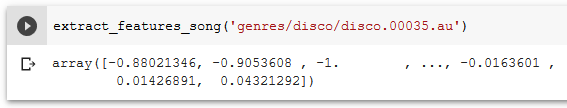
\includegraphics[width=8cm]{figures/1174006/chapter6/praktek/3-1.png}
		\centering
	\end{figure}
	Alasan diambil 25000 baris pertama, karena setiap lagu memiliki panjang nilai MFCC yang berbeda-beda dan yang dimasukkan ke dalam neuron harus memiliki ukuran yang sama.
	\item Jelaskan perbaris kode program dengan kata-kata dan dilengkapi ilustrasi gambar fungsi dari generatefeaturesandlabels().
	\hfill\break
	Kode program pada fungsi generate\_features\_and\_labels()
	\lstinputlisting[firstline=2, lastline=19]{src/1174006/chapter6/praktek/4.py}
	\begin{itemize}
		\item Disini nama fungsinya adalah generate\_features\_and\_labels().
		\item Membuat list all\_features
		\item Membuat list all\_labels
		\item Membuat list genres untuk menampung jenis-jenis genre musik
		\item Melakukan iterasi pada genres
		\item Panggil fungsi glob() untuk mencari list lagunya sesuai genre
		\item Menampilkan panjang list lagunya sesuai genrenya
		\item Melakukan itersai pada sound\_files
		\item Panggil fungsi extract\_features\_song()
		\item tambahkan hasil dari fungsi extract\_features\_song() ke all\_features
		\item Tambahkan genre ke all\_labels
		\item Panggil fungsi unique untuk menampilkan label unik
		\item Panggil fungsi astype untuk mengubah type sebelumnya ke type int32
		\item Panggil fungsi to\_categorical untuk mengubah ke one-hot-encoding
		\item Mengembalikan hasil fungsi stack() yaitu penggabungan dari all\_features ke matrix
	\end{itemize}
	\hfill\break
	\begin{figure}[H]
		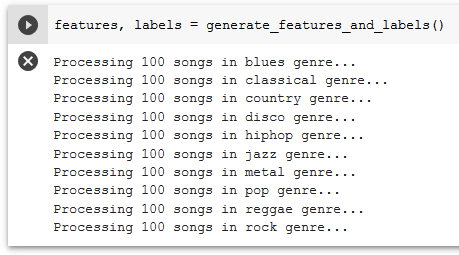
\includegraphics[width=8cm]{figures/1174006/chapter6/praktek/4-1.png}
		\centering
	\end{figure}
	\item Jelaskan dengan kata dan praktek kenapa penggunaan fungsi generate\_features\_and\_labels() sangat lama ketika meload dataset  genre. Tunjukkan keluarannya dari komputer sendiri dan artikan maksud setiap luaran yang didapatkan.
	\hfill\break
	Penggunaan fungsi generate\_features\_and\_labels() sangat lama ketika meload dataset genre karena datanya ada 1000 file dan kita mencari 25000 nilai dari mfccnya serta kita juga menggunakan one-hot encoding.
	\hfill\break
	\begin{figure}[H]
		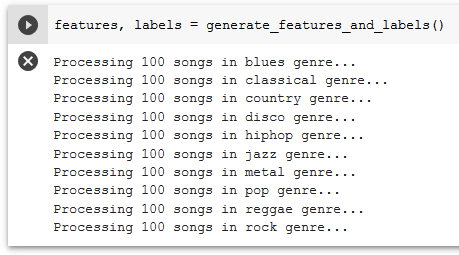
\includegraphics[width=8cm]{figures/1174006/chapter6/praktek/4-1.png}
		\centering
	\end{figure}
	\item Jelaskan kenapa harus dilakukan pemisahan data training dan data set sebesar 80 persen? Praktekkan dengan kode dan Tunjukkan keluarannya dari komputer sendiri dan artikan maksud setiap luaran yang didapatkan.
	\hfill\break
	Dilakukannya pemisahan data training dan data set sebesar 80 persen agar model yang dihasilkan lebih akurat dan meminimalisir kesalahan dalam pembelajaran mesin.
	\lstinputlisting[firstline=2, lastline=17]{src/1174006/chapter6/praktek/6.py}
	\hfill\break
	\begin{figure}[H]
		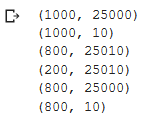
\includegraphics[width=8cm]{figures/1174006/chapter6/praktek/6-1.png}
		\centering
	\end{figure}
	\begin{itemize}
		\item Dimensi pada data features
		\item Dimensi pada data labels
		\item Dimensi pada data train
		\item Dimensi pada data test
		\item Dimensi pada data train\_input
		\item Dimensi pada data train\_labels
	\end{itemize}
	\item Praktekkan dan jelaskan masing-masing parameter dari fungsi Sequential(). Tunjukkan keluarannya dari komputer sendiri dan artikan maksud setiap luaran yang didapatkan.
	\hfill\break
	Parameter dari fungsi Sequential()
	\begin{itemize}
		\item Layer pertama akan menjadi layer dense dari 100 neuron, masukan dimensi dari data inputannya
		\item Menjalankan activation tipe relu
		\item Layer kedua outputnya menjadi 10 neuron
		\item Menjalankan activation tipe softmax
	\end{itemize}
	\lstinputlisting[firstline=2, lastline=7]{src/1174006/chapter6/praktek/7.py}
	\hfill\break
	\begin{figure}[H]
		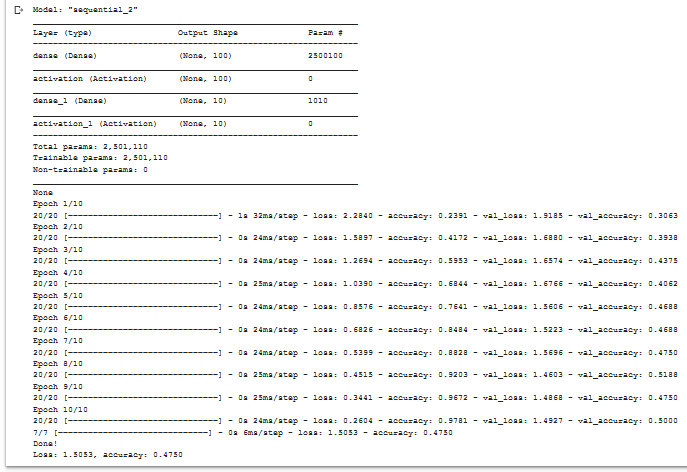
\includegraphics[width=8cm]{figures/1174006/chapter6/praktek/7-1.png}
		\centering
	\end{figure}	
	Output layer dense pertama ada 100 neuron dengan parameter 25000 input ditambah biasnya 100, output layer dense kedua ada 10 neuron dengan parameter 1000 input ditambah biasnya 10. Sehingga total parameternya ada 2501110. Kemudian dilakukan training.
	\item Praktekkan dan jelaskan masing-masing parameter dari fungsi compile(). Tunjukkan keluarannya dengan fungsi summary dari komputer sendiri dan artikan maksud setiap luaran yang didapatkan.
	\hfill\break
	\lstinputlisting[firstline=8, lastline=11]{src/1174006/chapter6/praktek/7.py}
	\begin{itemize}
		\item Optimizer yang diterapkan adalah adam
		\item Loss yang diterapkan adalah categorical\_crosssentropy
		\item Metrics yang diterapkan adalah accuracy
	\end{itemize}
	\hfill\break
	\begin{figure}[H]
		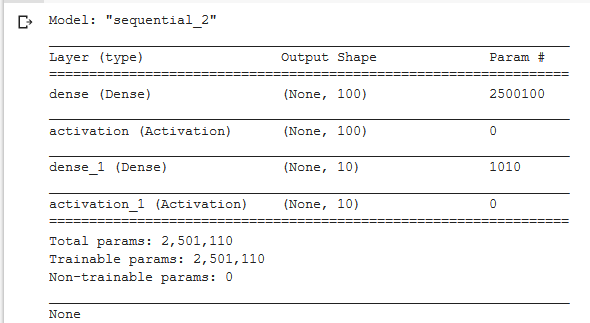
\includegraphics[width=8cm]{figures/1174006/chapter6/praktek/8-1.png}
		\centering
	\end{figure}
	Output layer dense pertama ada 100 neuron dengan parameter 25000 input ditambah biasnya 100, output layer dense kedua ada 10 neuron dengan parameter 1000 input ditambah biasnya 10. Sehingga total parameternya ada 2501110.
	\item  Praktekkan dan jelaskan masing-masing parameter dari fungsi fit().Tunjukkan keluarannya dari komputer sendiri dan artikan maksud setiap luaran yang didapatkan.
	\hfill\break
	\lstinputlisting[firstline=12, lastline=12]{src/1174006/chapter6/praktek/7.py}
	\begin{itemize}
		\item Parameter pertama data input train
		\item Parameter kedua data label train
		\item Epoch yang dibutuhkan 10
		\item Batch Size yang dibutuhkan 32
		\item Validation Splitnya 20\%
	\end{itemize}
	\hfill\break
	\begin{figure}[H]
		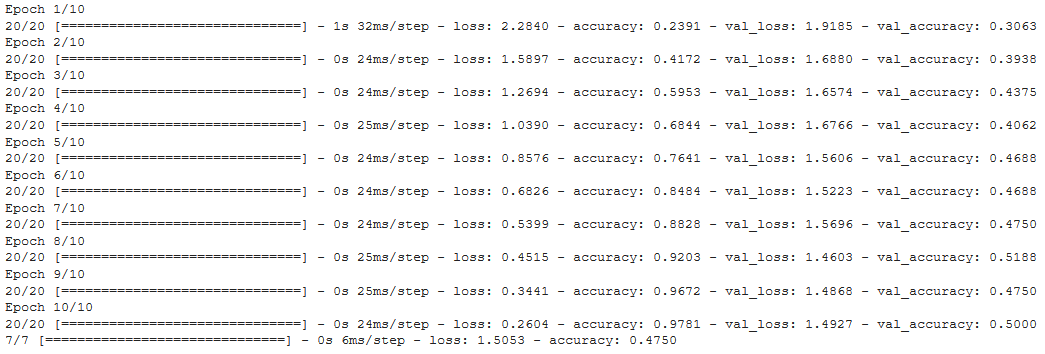
\includegraphics[width=8cm]{figures/1174006/chapter6/praktek/9-1.png}
		\centering
	\end{figure}
	Epoch yang dilakukan sebanyak 10 kali.
	\item Praktekkan dan jelaskan masing-masing parameter dari fungsi evaluate(). Tunjukkan keluarannya dari komputer sendiri dan artikan maksud setiap luaran yang didapatkan.
	\hfill\break
	\lstinputlisting[firstline=15, lastline=17]{src/1174006/chapter6/praktek/7.py}
	\begin{itemize}
		\item Parameter pertama data input test
		\item Parameter kedua data label test
		\item Batch Size yang dibutuhkan 32
	\end{itemize}
	\hfill\break
	\begin{figure}[H]
		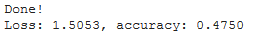
\includegraphics[width=8cm]{figures/1174006/chapter6/praktek/10-1.png}
		\centering
	\end{figure}
	Rata-rata loss yang didapat 1.5053, dan rata-rata akurasi yang didapat 0.4750
	\item Praktekkan dan jelaskan masing-masing parameter dari fungsi predict(). Tunjukkan keluarannya dari komputer sendiri dan artikan maksud setiap luaran yang didapatkan.
	\hfill\break
	\lstinputlisting[firstline=19, lastline=20]{src/1174006/chapter6/praktek/7.py}
	\begin{itemize}
		\item Parameter pertama data input test
		\item Batch Size yang dibutuhkan 32
	\end{itemize}
	\hfill\break
	\begin{figure}[H]
		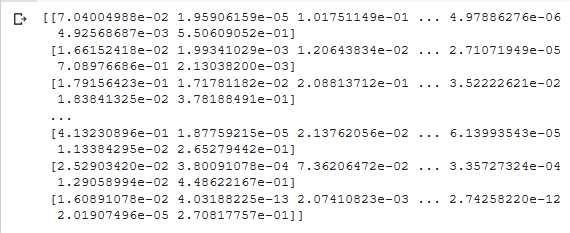
\includegraphics[width=8cm]{figures/1174006/chapter6/praktek/11-1.png}
		\centering
	\end{figure}
\end{enumerate}

\subsection{Penanganan Error}

\subsection{Bukti Tidak Plagiat}
\begin{figure}[H]
	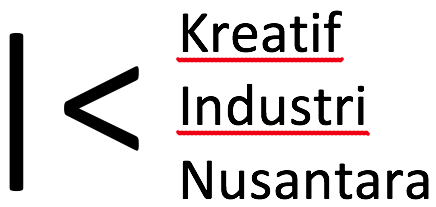
\includegraphics[width=8cm]{kreatiflogo.png}
	\centering
	\caption{Kecerdasan Buatan.}
\end{figure}